\section{Supporting Mathematics}\label{app.model.math}
%===================================================================================================
\subsection{Exponential Duration Assumption in Compartmental Models}\label{app.model.math.exp}
Let $\lambda$ be the fixed exit rate from compartment $A$, which is assumed to be homogeneous.
Then $\delta \sim \lambda e^{-\lambda \delta}$ is % TODO: double check this
the exponentially distributed duration time in the group.
\paragraph{Mean \& Median Duration}
The mean duration is $\mu = 1/\lambda$ and the median is $m = \log(2)/\lambda \approx 0.69\,\mu$.
Thus, if 50\% of individuals progress from compartment $A$ to $B$ by time $\tau$ (median duration),
the exit rate $\lambda$ is given by $\log(2)/\tau$.
\paragraph{Collapsing Compartments in Series}
Let compartments $A$ and $B$ be in series, with exit rates $\lambda_A$ and $\lambda_B$ respectively.
Collapsing $A$ and $B$ into $AB$ will sum the mean durations: $\delta_{AB} = 1/\lambda_A + 1/\lambda_B$;
thus, the exit rate from $AB$ will be $\lambda_{AB} = 1/(1/\lambda_A + 1/\lambda_B)$.
\paragraph{Collapsing Compartments in Parallel}
Let compartments $A$ and $B$ be in parallel, with exit rates $\lambda_A$ and $\lambda_B$ respectively.
Collapsing $A$ and $B$ into $AB$ will sum the exit rates: $\lambda_{AB} = \lambda_A + \lambda_B$;
thus, the mean duration in $AB$ will be $\delta_{AB} = 1/(\lambda_A + \lambda_B)$.
%===================================================================================================
\subsection{Beta Approximation of the Binomial (BAB) Distribution}\label{app.model.math.bab}
Numerous model parameters and calibration targets represent population proportions.
Such proportions can be estimated as $\rho = n / N$, where
$N$ is the sample size and $n$ is the number of individuals with the characteristic of interest.
The uncertainty around $n$ is then given by the binomial distribution:
\begin{equation}\label{eq:binom}
  p(n) = {N \choose n} \, \rho^{n}{(1 - \rho)}^{N - n}
\end{equation}
However, \eqref{eq:binom} is only defined for discrete values of $n$.
It is more convenient to have a continuous distribution for $\rho$,
for sampling parameters and evaluating the likelihood of calibration targets,
since compartmental models can have non-whole-number population sizes.
For this purpose, I use a beta approximation of the binomial distribution (BAB):
\begin{equation}\label{eq:beta}
  p(\rho) =
    \frac{\Gamma(\alpha+\beta)}{\Gamma(\alpha)\,\Gamma(\beta)}\,
    \rho^{\alpha-1}{(1 - \rho)}^{\beta-1}
\end{equation}
with $\alpha = N\,\rho$ and $\beta = N\,(1-\rho)$.
Unlike the approximation by a normal distribution,
the beta distribution ensures that $\rho \in [0,1]$.
Figure~\ref{fig:bab} illustrates the approximation for
$N = \{10,20,40\}$ and $\rho = \{0.01,0.1,0.5\}$.
\begin{figure}
  \centering
  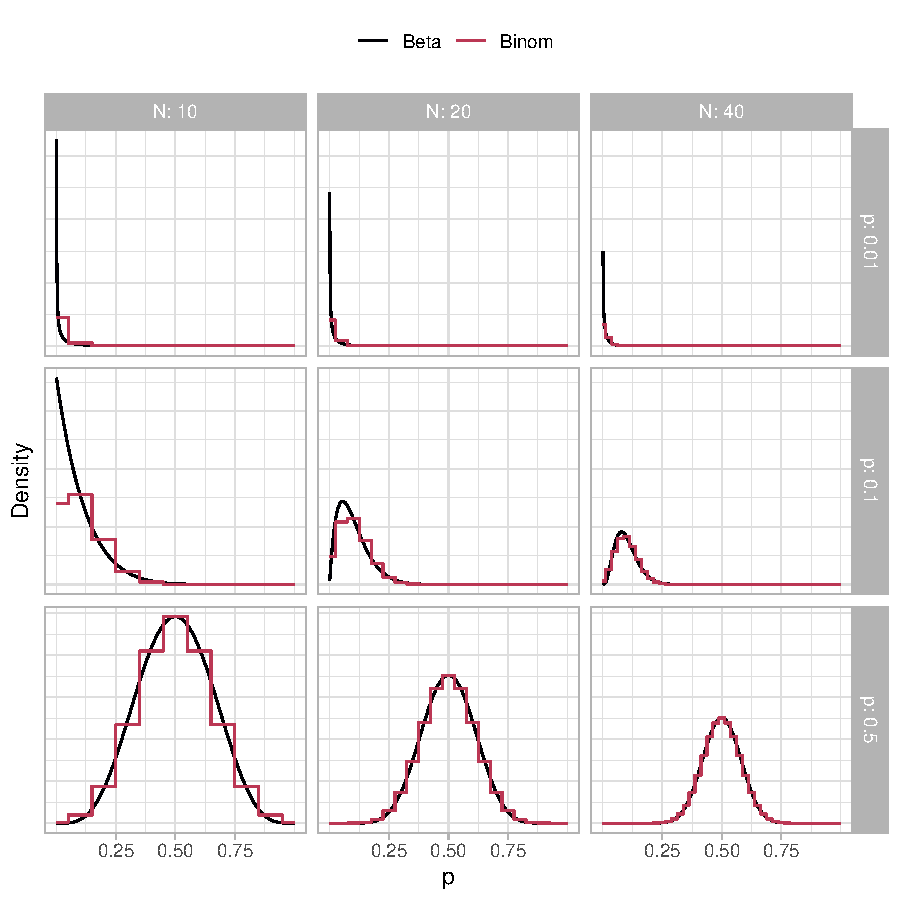
\includegraphics[width=.8\linewidth]{bab}
  \caption{Beta approximation of the binomial distribution (BAB)}
  \label{fig:bab}
\end{figure}
%===================================================================================================
\subsection{Joint Sampling with Relational Constraints}\label{app.model.math.jsam}
Figure~\ref{fig:jsam.bias} illustrates the posterior (sampled) distributions
for variables $X_1$, $X_2$, $X_3$, having uniform priors but subject to $X_1 < X_2 < X_3$.
Three approachs to enforcing $X_1 < X_2 < X_3$ were explored:
\begin{itemize}
  \item \textbf{joint:}
    sample $X_1$, $X_2$, $X_3$ simultaneously;
    then discard any samples failing $X_1 < X_2 < X_3$.
  \item \textbf{forward:}
    sample $X_1$;
    then sample $X_2$ until $X_1 < X_2$;
    then sample $X_3$ until $X_2 < X_3$.
  \item \textbf{backward:}
    sample $X_3$;
    then sample $X_2$ until $X_2 < X_3$;
    then sample $X_1$ until $X_1 < X_2$.
\end{itemize}
All three methods result in a different posterior \vs the prior,
but the forward and backward methods
severely distort the distributions for $X_3$ and $X_1$, respectively,
while leaving the distributions for $X_1$ and $X_3$ unchanged.
By contrast, the joint method influences the posterior distributions of each variable
in a more ``equitable'' way, which is preferred.
\begin{figure}[h]
  \centering
  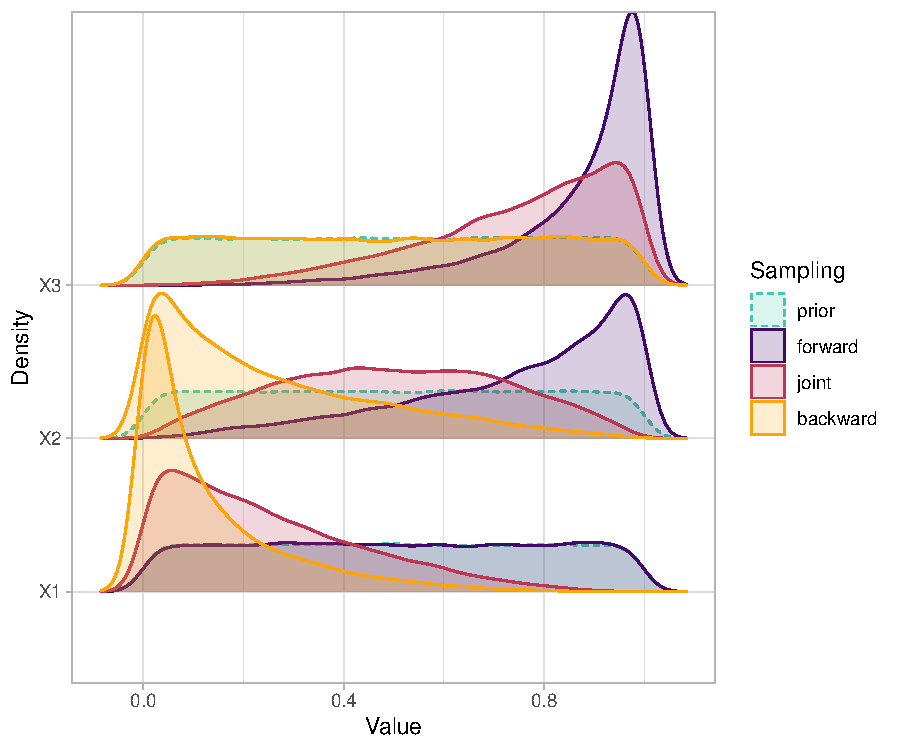
\includegraphics[width=.6\linewidth]{jsam.bias}
  \caption{Illustration of different sampling biases when enforcing $X_1 < X_2 < X_3$}
  \label{fig:jsam.bias}
\end{figure}
%===================================================================================================
\subsection{Fitting Distributions}\label{app.model.math.fit}
Uncertainty distributions for all parameters and calibration targets were estimated by
fitting a parametric distribution to specified quantiles.
Let $f\,(x\mid\theta)$ be
the probability density function of random variable~$x$ (parameter or target)
given distribution parameters $\theta$.
Then $F\,(x\mid\theta) = \int_0^x f(\tau)\,d\tau$ is the cumulative distribution function,
and $Q(p\mid\theta) = F^{\,-1}(p\mid\theta)$ is the quantile function.
Our objective is to estimate $\theta$, given a set of quantiles
(\eg $q = \{q_{2.5},q_{97.5}\}$ for the 95\%~CI).
For each estimation, I minimized%
\footnote{Using \hreftt{docs.scipy.org/doc/scipy/reference/optimize.minimize-lbfgsb.html}}
the following error function:
\begin{equation}
  J\,(\theta) = \sum_i {\big|\,q_i - Q(p_i\mid\theta)\,\big|}^{\,\omega}
\end{equation}
where $\omega$ can specify absolute differences ($\omega=1$) or squared differences ($\omega=2$)
to improve convergence.
Distribution fit was validated visually using a plot of
the distribution quantiles $Q(p_i\mid\theta)$ \vs the target quantiles $q_i$,
overlaid on the density distribution $f\,(x\mid\theta)$; \eg Figure~\ref{fig:distr.fit}.
\begin{figure}[h]
  \centering
  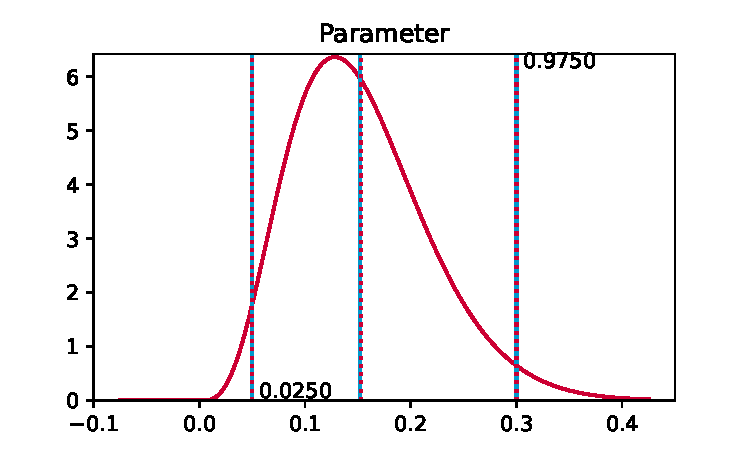
\includegraphics[width=.6\linewidth]{distr.fit}
  \caption{Example distribution fitting validation plot}
  \label{fig:distr.fit}
  \floatfoot{BAB distribution fit to $\{q_{2.5} = .05, q_{97.5} = .30\}$;
    blue solid lines: target quantiles $q_i$;
    red dotted lines: distribution quantiles $Q(p_i\mid\theta)$;
    red solid line: density distribution $f\,(x\mid\theta)$.}
\end{figure}
%===================================================================================================
\subsection{Estimating Duration in Sex Work from Cross Sectional Data}\label{app.model.math.xdur}
Cross sectional sex work surveys will often ask respondents about their duration in sex work.
These durations might then be taken to be the average durations in sex work;
however, this will be an underestimate,
because respondents will continue selling sex after the survey \cite{Fazito2012}.%
\footnote{An alternate example would be
  to take the mean age of a population as the life expectancy!
  Thanks to Saulius Simcikas and Dr. Jarle Tufto
  for help identifying and discussing this bias:
  \hreftt{stats.stackexchange.com/questions/298828}.}
% TODO: (?) This bias parallels challenges to estimating sexual partnership duration \cite{Burington2010}.
\par
Figure~\ref{fig:diag.xdur} illustrates a steady-state population
with 4 women selling sex at any given time.
The steady-state assumption implies that a women leaving sex work after $\delta$ years
will be immediately replaced by a women entering sex work
whose eventual duration will also be $\delta$ years.
Let $\delta$ be this true duration, and $\delta_s$ be the duration reported in the survey.
If we assume that the survey reaches women at a random time point during the duration $\delta$,
then $\delta_s \sim \opname{Unif}(0,\delta)$,
and the mean reported duration is $E(\delta_s) = \frac{1}{2}E(\delta)$.
Thus, $E(\delta) = 2 E(\delta_s)$ would be an estimate of the true mean duration from the sample.
In reality, sex work surveys may be more likely to reach
women who have already been selling sex for several months or years,
due to delayed self-identification as sex worker \cite{Cheuk2020}.
Thus, we would expect that $f = E(\delta) / E(\delta_s) \in (1,2)$,
which we can use to compute the mean exit rate as described in \sref{app.model.math.exp}.
\begin{figure}[h]
  \centering
  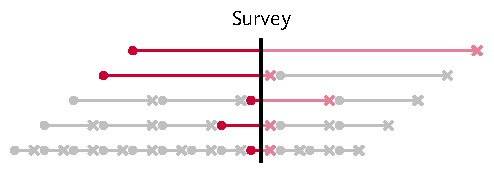
\includegraphics[scale=1]{diag.xdur}
  \caption{Illustrative steady-state population of 4 FSW,
    with varying true durations in sex work $\delta$,
    \vs the observed durations in sex work $\delta_s$ via cross-sectional survey.}
  \label{fig:diag.xdur}
\end{figure}
\par
Another observation we can make from Figure~\ref{fig:diag.xdur} is that
women who sell sex longer are more likely to be captured in the survey.
That is, while the sampled durations are representative of women who \emph{currently} sell sex,
these durations are biased high \vs the population of women who \emph{ever} sell sex.
It's not clear whether this observation is widely understood
and kept in mind when interpreting sex work survey data.
%===================================================================================================
\subsection{Quantifying Partnerships}\label{app.model.math.qp}
Similar to \sref{app.model.math.xdur},
sexual partnerships are often quantified using cross-sectional surveys.
In this case, respondents are typically asked to report the numbers of unique partners ``$x$''
during a standardized recall period $\omega$ --- \eg
\shortquote{How many different people have you had sex with during the past year?}
Such data can then be used to inform modelled
rates of partnership change $Q$ and/or numbers of concurrrent partnerships $K$.
\par
If partnership duration is long and the recall period is short
--- including $\omega \approx 0$ for
\shortquote{Are you currently in a long-term sexual partnership?} ---
the reported partnerships mostly reflect \emph{ongoing} partnerships,
and thus $x \approx K$.
If partnership duration is short and the recall period is long,
--- including $\delta \approx 0$ for
\shortquote{How many one-off sexual partners have you had during the past year?} ---
the reported partnerships mostly reflect \emph{complete} partnerships,
and thus $x/\omega \approx Q$.
However, if partnership duration and recall period are similar in length,
the reported partnerships reflect a mixture of tail-ends, complete, and ongoing partnerships,
and thus $x$ overestimates $K$, but $x/\omega$ also overestimates $Q$.
In summary:
\begin{itemize}
  \item $\omega \ll \delta$: mostly ongoing partnerships;
  $x \approx K$ (concurrrent)
  \item $\omega \gg \delta$: mostly complete partnerships;
  $x/\omega \approx Q$ (change rate)
  \item $\omega\,\approx\,\delta$: some tail-ends, some complete, some ongoing;
  $x > K$, $x/\omega > Q$ (neither)
\end{itemize}
\par
I developed an approach to estimate $Q$ and $K$ from $x$ and $\omega$.
The approach draws on a similar assumption as in \sref{app.model.math.xdur}:
that survey timing is effectively random with respect to partnership duration.
Then, if either end of the recall period would capture an ongoing partnership,
the intersection point would be, on average, at the partnership mid-point.
Thus, the recall period is effectively extended
by half the partnership duration $\delta/2$ on each end, and $\delta$ overall,
as illustrated in Figure~\ref{fig:diag.recall}.
As such, we can define $Q$ and $K$ as:
\begin{alignat}{1}
  Q &= \frac{x}{\omega+\delta} \label{eq:C2Q.app}\\
  K &= \frac{x\delta}{\omega+\delta} = Q\delta \label{eq:C2K.app}
\end{alignat}
\begin{figure}
  \centering
  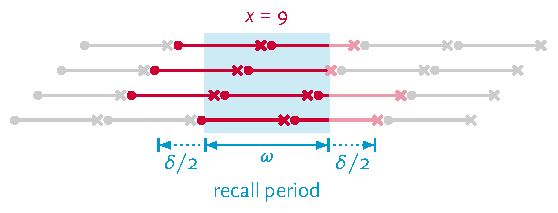
\includegraphics[scale=1]{diag.recall}
  \caption{Illustration of conceptual framework for quantifying partnerships
    from the number reported during a given recall period}
  \label{fig:diag.recall}
  \floatfoot{
    Circle: partnership start; line: ongoing partnership; cross: partnership end;
    $\omega$/red: recall period;
    $\delta$: partnership duration;
    $x$: number of reported partnerships for $\omega$.}
\end{figure}
\par
As an example, Figure~\ref{fig:diag.recall} illustrates
a recall period of $\omega = 1$ year,
for which $x = 9$ partnerships are reported,
having durations of $\delta = 9$ months.
Thus, we can compute $Q = 9/(1+0.75) = 5.14$ and $K = 5.14(0.75) = 3.86$,
which is a slight underestimate of the true values $Q = 5.33, K = 4$,
due to the randomness in the exact ``location'' of the recall period.

